% !TEX root = ../main.tex

% 中英标题：\chapter{中文标题}[英文标题]

\chapter{主要研究内容及研究方案}

\section{研究内容}
基于多模态预训练的蛋白质功能预测研究旨在通过结合深度学习和多种生物信息数据来源（如序列数据、结构数据和功能标注），提高预测精度，尤其是在未见功能标签上的预测能力。利用如AlphaFold2等结构预测工具的突破，以及其他相关生物信息技术的进展，本研究将探索如何有效地整合这些多模态数据来增强蛋白质功能的预测效果。研究的具体内容包括：

（1）设计并实现一个双分支VAE\cite{kingma2013auto}预训练模型，用于同时编码蛋白质的序列和结构特征。序列和结构分别通过独立的编码器分支进行处理，并通过预训练提取出通用低维蛋白质特征表示。

（2）在VAE生成的蛋白质特征表示基础上，使用扩散模型进行GO标签的分类。扩散模型的优势在于它能够处理未见过的功能标签，通过生成过程估计各个类别的条件概率。

（3）在包含未见功能标签的测试集上对模型进行评估，验证其蛋白质功能预测能力。通过与其他传统方法（如基于序列相似性的方法）的对比实验，展示该模型在处理稀有功能标签上的优势。

\section{研究方案}
\subsection{获取并整合数据集}
本课题的研究内容涉及到蛋白质的序列、结构和功能标签三种数据，其中序列来自UniProt数据库\cite{uniprot2023uniprot}，结构来自AlphaFold数据库\cite{varadi2022alphafold}，功能标签集合来自基因本体注释（GOA）数据库\cite{huntley2015goa}。UniProt是一个广泛使用的蛋白质数据库，包括各种重要部分,UniProt版本2024\_01包含超过2.5亿个序列记录。UniProt手动管理和审查条目的部分被称为UniProtKB/Swiss-Prot\cite{boutet2016uniprotkb}，包含约570 000个序列。未经审查的部分被称为UniProtKB/TrEMBL，包含约2.49亿个序列。根据CAFA，不具实验性注释的蛋白质的注释是电子化的（证据代码：IEA），可能包含潜在的错误，为了保证模型的泛化性，我们在UniProtKB/Swiss-Prot中选择了不具实验性注释的508245个蛋白质进行预训练。带有证据代码（EXP、IDA、IPI、IMP、IGI、IEP、TAS和IC）的注释被认为是实验性的，为了确保实验结果的准确性和可靠性，我们选择了带有实验证据代码的60121个蛋白质在下游预测中进行微调。并使用GO\cite{ashburner2000gene}的分层结构传播注释。

AlphaFold是DeepMind和EMBL-EBI共同开发的高精度蛋白质结构预测数据库，在v2.0版本中，它包含超过2亿个条目，包括48种关键生物的蛋白质组，提供了广泛的UniProt覆盖范围。对于数据库中未包含的蛋白质结构，可以使用源代码（https：//github.com/google-deepmind/alphafold/）进行结构预测。为保证不同数据的蛋白质节点之间的映射对齐，本课题还下载了Uniprot映射到AlphaFold的映射文件。

基因本体注释（GOA）为UniProt知识库（UniProtKB）中的蛋白质提供高质量的GO注释。GOA采用两种不同的GO注释方法：电子和手动\cite{barrell2009goa}。目前GOA标注总数超过13.77亿条，其中电子GO标注约13.72亿条，人工GO标注仅约590万条。具体而言，GOA数据库中超过99\%的GO注释是通过电子注释方法进行的。GOA数据库中有不同来源的功能注释信息，为了GO标签的真实可靠，本课题筛选了具有实验验证和专家手工收集的功能注释。

\begin{table}[h]
\centering
\caption{时间流数据集划分方法}
\begin{tabular}{@{}cc@{}}
\toprule
\textbf{数据集} & \textbf{划分依据} \\ \midrule
训练集 & 2021年1月之前就具有实验注释的蛋白质 \\ 
验证集 & 2021年1月至2022年12月期间首次获得实验注释的蛋白质 \\ 
测试集 & 2023年1月至2024年7月期间首次获得实验注释的蛋白质 \\ \bottomrule
\end{tabular}
\end{table}

下游数据集划分共包含依据时间流划分和基于序列相似性聚类的两种策略，依据时间流划分数据集的方法如表3-1所示。为了验证本课题所提出的方法对于序列同源相似性低的蛋白质功能标签的预测能力，还对原始蛋白质数据进行了基于序列相似性的初始聚类步骤。为了确保所得簇之间的独特性，任何两个簇之间的序列相似性被限制为最大30\%，随后分别按照18：1：1的比例划分训练集、验证集和测试集。

\subsection{构建双分支VAE预训练框架}
国内外学者已经在蛋白质序列的低维表示上做了很多研究工作，有近两年兴起预训练语言模型的方法，例如esm3\cite{hayes2024simulating}、SaProt\cite{su2023saprot}、ProGen\cite{madani2020progen}等；有较老的CNN\cite{li2021survey}、LSTM\cite{yu2019review}等方法；还有类似InterProScan\cite{jones2014interproscan}等工具，这些方法已经能够提取到序列特征的关键信息，如蛋白质家族、结构域、结合位点等。本课题计划采用与当前蛋白质语言模型类似的模块对序列进行编码提取有效信息。

随着AlphaFold2\cite{bryant2022improved}的巨大突破，越来越多的蛋白质能用来进行蛋白质功能预测，为了方便蛋白质结构的表示，出现了接触图的概念，基于接触图的方法能够简化蛋白质结构的初步表示，便于进一步通过深度学习提取蛋白质的结构特征产生低维表示，但通常是计算昂贵的。点云是一种常用的3D数据格式，在包括计算机视觉、自动驾驶和机器人技术在内的许多领域都取得了巨大成功\cite{guo2020deep}。点云可以表示为一组无序的3D点$\{P_i \mid i = 1, \ldots, n\}$，其中所有点都是齐次的，并且每个点$P_i$是其\( (x, y, z) \)坐标的向量。与接触图和蛋白质图相比，点云具有在不牺牲计算效率的情况下保留原子几何信息的优点。与无序且同质的原始点云相比，我们计划采用的蛋白质点云由从其原始结构中提取的有序和异质点组成，具体来说每个点对应于氨基酸的α碳原子。除了每个点的3D坐标 \((x, y, z)\) 之外，每个点所属的残基类型 \(R\) 以及该残基在长度为 \(L\) 的蛋白质序列中的位置 \(P\) 也被附加为点特征。蛋白质点云中每个点的定义为：$[x, y, z, R, P]$，
\(R \in (\text{G, A, V, L, I, S, T, C, M, D, E, N, Q, R, K, F, Y, W, P, H})\)，
\(P \in (1, 2, 3, \ldots, L)\)。

\begin{figure}[h]
\centering
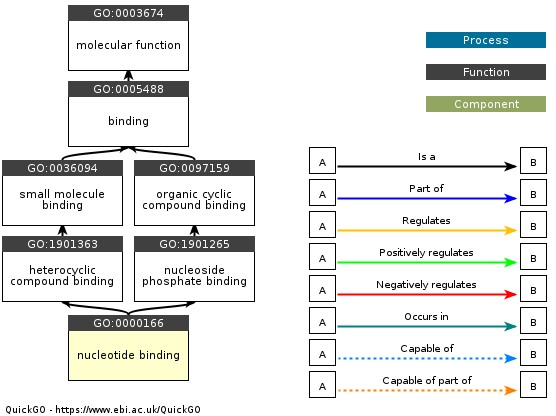
\includegraphics[width = 1\textwidth]{figures/1.jpg}
\caption{GO树状结构示例\cite{binns2009quickgo}}
\label{fig:go}
\end{figure}

功能标签，即GO标签，它们之间并不是独立或者简单集合的关系，而是一种树状结构关系，如图3-1所示。所有的GO标签都在这个树状结构的基因本体库中。基因本体库不重叠地分为三个分支\cite{gene2004gene}：细胞组分（Cellular Component，CC），单个的基因产物或多个基因产物的复合物在分子水平上的活动；分子功能（Molecular Function，MF），基因产物在执行功能时所处的细胞结构位置；生物过程（Biological Process，BP）， 通过多种分子活动完成的生物学过程。在每个子系统内，所有的节点形成了有向无环图。并且，GO子节点与父节点之间存在着“is a”和“part of”关系，这意味着如果一个蛋白质拥有某个GO节点表示的功能，那么也拥有该GO节点的父节点表示的功能。基于GO的这种真正路径规则，GO标签在进行嵌入之前，还需要向上传播进行标签补全，否则会产生标签不一致等问题。之后对每一个蛋白质的标签集合编码，利用深度学习产生合适的嵌入表示作为扩散模型的类条件输入。

\begin{figure}[h]
\centering
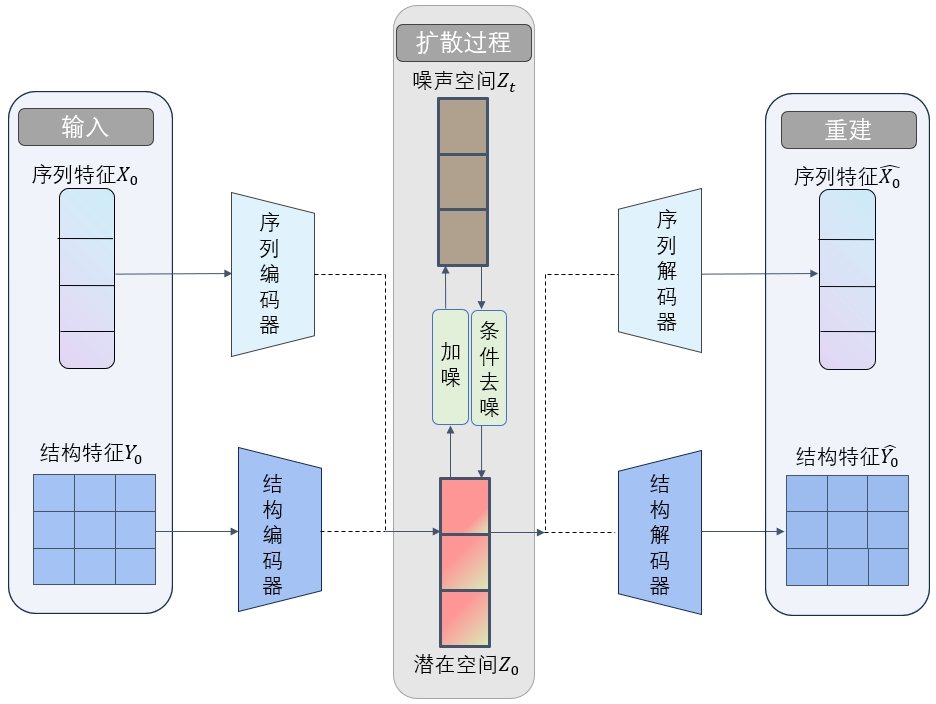
\includegraphics[width = 1\textwidth]{figures/pre.png}
\caption{双分支VAE预训练框架示意图}
\label{fig:pretrain}
\end{figure}

本课题计划采用一种创新的双分支编码器-解码器变分自编码器（VAE）预训练架构，旨在同时处理和学习来自蛋白质序列、结构与功能注释的信息，双分支VAE预训练的模型架构如图3-2所示。这一架构通过分别对序列上下文和结构上下文进行编码，将两个不同模态的特征有效地整合并映射到统一的潜在向量空间中，进一步采用加噪与类条件去噪扩散过程对融合功能注释的向量分布进行学习，最后分别根据交叉熵（CE）损失与Chamfer距离（CD）损失评估网络性能重建蛋白质序列与结构。该预训练旨在增强对蛋白质数据通用表示的学习能力，提高其在复杂生物数据中的泛化能力，为下游的功能预测和其他生物信息学处理任务提供强大的数据支持。

\subsection{构建扩散模型网络}
本课题计划构建一个扩散模型网络，旨在提高蛋白质功能预测的准确性和泛化能力，输入为蛋白质序列和结构的潜在空间特征。
扩散模型是一类具有特定马尔可夫链结构的生成模型，本课题计划采用离散时间扩散模型的设计思想\cite{hoogeboom2021argmax}。从一个干净的样本 \( z_0 \) 开始，固定的前向过程 \( q(z_t | z_{t-1}) \) 添加高斯噪声，而学习到的反向过程 \( p_\theta(z_{t-1} | z_t, c) \) 尝试对输入去噪，可选地基于一个变量 \( c \) 进行条件化。在我们的设置中，\( z \) 是蛋白质的潜在空间表示，而 \( c \) 代表一个低维的蛋白质GO功能标签嵌入。扩散模型定义 \( z_0 \) 的条件概率为\cite{kingma2021variational}：
\begin{equation}
p_\theta(z_0 | c) = \int p(z_T) \prod_{t=1}^{T} p_\theta(z_{t-1} | z_t, c) \, dz_{1:T}
\end{equation}

其中 \( p(z_T) \) 通常固定为 \( \mathcal{N}(0, \mathbf{I}) \)。由于直接最大化 \( p_\theta(z_0) \) 涉及积分运算，难以实现，因此扩散模型通过最小化对数似然的变分下界（ELBO\cite{song2020score}）进行训练：
\begin{equation}
\log p_\theta(z_0 | c) \geq \mathbb{E}_q \left[\log \frac{p_\theta(z_{0:T}, c)}{q(z_{1:T} | z_0)}\right]
\end{equation}

扩散模型将 \( p_\theta(z_{t-1} | z_t, c) \) 参数化为高斯分布，并训练一个神经网络，将带噪声的输入 \( z_t \) 映射到用于计算 \( p_\theta(z_{t-1} | z_t, c) \) 均值的值。每个带噪声的样本 \( z_t = \sqrt{\bar{\alpha}_t} z + \sqrt{1 - \bar{\alpha}_t} \epsilon \) 可以表示为一个干净输入 \( z \) 和高斯噪声 \( \epsilon \sim \mathcal{N}(0, \mathbf{I}) \) 的加权组合，扩散模型通常会学习一个网络 \( \epsilon_\theta(z_t, c) \) 来估计添加的噪声\cite{sohl2015deep}。使用这种参数化，ELBO 可以写为：
\begin{equation}
-\mathbb{E}_\epsilon \left[\sum_{t=2}^{T} w_t \|\epsilon - \epsilon_\theta(z_t, c)\|^2 - \log p_\theta(z_0 | z_1, c)\right] + C
\end{equation}

其中 \( C \) 是一个不依赖于 \( c \) 的常数项。由于 \( T\) 很大且 \( \log p_\theta(z_0 | z_1, c) \) 通常较小，因此选择忽略这一项。研究发现发现去掉 \( w_t \) 可以改善样本质量指标\cite{ho2020denoising}，于是ELBO的最终表达式为：
\begin{equation}
-\mathbb{E}_{t, \epsilon} \left[\|\epsilon - \epsilon_\theta(z_t, c)\|^2\right] + C
\end{equation}

扩散模型通过其生成过程学习数据的底层分布，而不仅仅是记忆训练数据中的特定模式。这种学习方式使模型能够更好地泛化到未见过的蛋白质序列或结构，特别是那些在训练集中没有直接功能标签的蛋白质。本课题设计的扩散模型可以用于多种蛋白质功能预测任务，尤其是在新物种蛋白质功能注释、稀有功能标签发现等领域具有重要应用前景。通过将序列和结构特征有机结合，本课题为蛋白质功能预测提供了一种创新的解决方案，具有广泛的生物学和医学研究意义。

\subsection{扩散模型上的类条件分类器}
近年来，基于条件生成模型的分类方法在图像零样本分类方面展现出巨大潜力，本课题中使用扩散模型进行蛋白质功能预测的框架如图3-3所示。模型输入序列特征 \(X_0\) 和结构特征 \(Y_0\) ，分别通过序列编码器和结构编码器进行处理，得到潜在空间表示 \(Z_0\) 和结构特征表示。在此基础上将 \(Z_0\) 添加噪声后生成噪声空间表示 \(Z_t\)，接下来将 \(Z_t\) 输入到扩散模块中，该模块结合 GO 标签条件 \(c\) 进行键值查询操作，从而完成特征的扩散处理。通过这种方法，即使对于未见过的类别，也能通过标签条件 \(c\) 提供的语义信息进行准确分类。最后通过最小化采样噪声 \( \epsilon_{\theta} \) 和添加噪声 \( \epsilon \) 之间的损失函数，实现分类目标。该框架通过一系列编码、噪声添加、扩散处理步骤，最终精确预测输入数据的类别。
\begin{figure}[h]
\centering
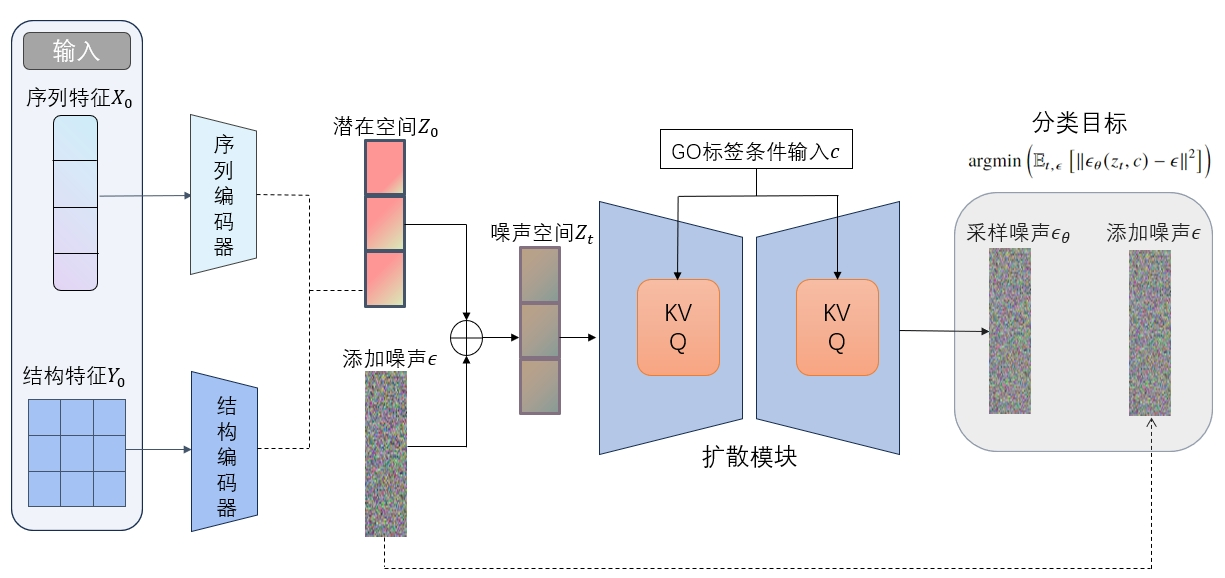
\includegraphics[width = 1\textwidth]{figures/class.png}
\caption{扩散分类器预测蛋白质功能框架示意图}
\label{fig:pretrain}
\end{figure}

具体而言，通过贝叶斯定理，利用模型预测结果和标签先验 \(p(c)\)，我们可以实现对给定输入 \(z\) 的条件概率 \(p_\theta(c_i \mid z)\) 的计算，对于标签集合 \(\{c_i\}\)，条件概率的计算公式如下：
\begin{equation}
    p_\theta(c_i \mid z) = \frac{p(c_i) p_\theta(z \mid c_i)}{\sum_j p(c_j) p_\theta(z \mid c_j)}
\end{equation}

在假设标签的先验分布为均匀分布（即 \(p(c_i) = \frac{1}{N}\)）的情况下，所有 \(p(c)\) 项可以相互抵消。对于扩散模型来说，直接计算 \(p_\theta(z \mid c)\) 是不可行的。因此我们使用变分下界（ELBO）来代替 \(\log p_\theta(z \mid c)\)，并结合以下公式来获得给定标签集合 \(\{c_i\}_{i=1}^N\) 的后验分布\cite{song2019generative}：
\begin{equation}
    p_\theta(c_i \mid z) = \frac{\exp\left(-\mathbb{E}_{t,\epsilon} \left[\|\epsilon - \epsilon_\theta(\mathbf{z}_t, c_i)\|^2\right]\right)}{\sum_j \exp\left(-\mathbb{E}_{t,\epsilon} \left[\|\epsilon - \epsilon_\theta(\mathbf{z}_t, c_j)\|^2\right]\right)}
\end{equation}

为了计算每个期望的无偏蒙特卡洛估计\cite{doucet2015efficient}，我们通过采样 \(N\) 对 \((t_i, \epsilon_i)\)，其中 \(t_i \sim [1, 1000]\) 且 \(\epsilon \sim \mathcal{N}(0, \mathbf{I})\)，并计算以下公式：
\begin{equation}
    \frac{1}{N} \sum_{i=1}^N \left\|\epsilon_i - \epsilon_\theta\left(\sqrt{\bar{\alpha}_{t_i}} \mathbf{z} + \sqrt{1 - \bar{\alpha}_{t_i}} \epsilon_i, c_j\right)\right\|^2
\end{equation}

通过将此公式代入上述后验分布的公式中，我们可以从条件扩散模型中提取分类器。扩散分类器是一种强大的、无需超参数调整的方法，可以从预训练的扩散模型中提取分类器，而无需进行额外的训练。扩散分类器可以用于从文本到图像模型（如Stable Diffusion\cite{rombach2022high}）中提取零样本分类器，或者从类条件扩散模型（如DiT\cite{peebles2023scalable}）中提取标准分类器。总之，本课题旨在利用扩散分类器这一创新方法，通过结合蛋白质序列和结构特征，实现更精确的蛋白质功能预测，推动蛋白质功能注释的零样本预测研究。
\renewcommand{\algorithmicrequire}{\textbf{输入:}}  
\renewcommand{\algorithmicensure}{\textbf{输出:}} 
\begin{algorithm}
\caption{基于扩散模型的蛋白质功能分类器}
\begin{algorithmic}[1]
\REQUIRE  蛋白质潜在空间表示$z$,蛋白质功能标签 $\{c_i\}_{i=1}^n$，每个输入的采样次数T
\ENSURE  预测的功能标签$Selectlabels$
\STATE 初始化 $\text{Labels}[c_i] = \text{list}()$ 对每个 $c_i$
\FOR{$j = 1, \ldots, T$}
    \STATE 从 $[1, 1000]$ 中采样 $t$； $\epsilon \sim \mathcal{N}(0, I)$
    \STATE 计算 $z_t = \sqrt{\bar{\alpha}_t}z + \sqrt{1 - \bar{\alpha}_t}\epsilon$
    \FOR{条件功能标签 $c_k \in \{c_i\}_{i=1}^n$}
        \STATE 将 $\|\epsilon - \epsilon_\theta(x_t, c_k)\|^2$ 加入到 $\text{Labels}[c_k]$ 中
    \ENDFOR
\ENDFOR
\STATE 对每个 $c_i$计算功能标签平均误差：$\text{MeanLabels}[c_i] = \text{mean}(Labels[c_i])$ 
\STATE 选择误差低于阈值的标签：$SelectedLabels = \{c_i \mid \text{MeanLabels}[c_i] < \text{threshold}\}$
\RETURN $Selectlabels$
\end{algorithmic}
\end{algorithm}
\subsection{优化多标签分类器及模型评估}
蛋白质功能预测是一个典型的多标签学习问题，与传统的分类问题相比较主要有标签之间相互依赖和标签数量不确定两个问题，对于前者，本课题使用真正路径规则在获取标签嵌入时解决；对于后者，关键是要设计并优化合适的多标签分类算法。本课题采用基于机器学习的多标签学习算法整合前述提取出的蛋白质节点表示，构建蛋白质功能预测模型。

为了从不同角度评估不同方法的预测准确性，我们选择了两种不同的度量标准，包括F-max分数（Fmax）和精确率-召回率曲线下面积（AUPR）。Fmax \cite{clark2013information} 是一种蛋白质中心的度量标准，在CAFA挑战赛 \cite{radivojac2013large} 和许多蛋白质功能预测研究中使用，其取值范围为0到1，其中1表示模型的最佳性能，0表示最差性能。其定义如下：

\begin{equation}
\text{Fmax} = \max_{\tau} \left(\frac{2 \times \text{pr}(\tau) \times \text{rc}(\tau)}{\text{pr}(\tau) + \text{rc}(\tau)}\right)
\end{equation}

$\text{pr}(\tau)$ 和 $\text{rc}(\tau)$ 分别是阈值 $\tau$ 下的精确率和召回率，其定义如下：

\begin{equation}
\text{pr}(\tau) = \frac{1}{m(\tau)} \sum_{i=1}^{m(\tau)} \frac{\left|P_i(\tau) \cap T_i\right|}{\left|P_i(\tau)\right|}
\end{equation}

\begin{equation}
\text{rc}(\tau) = \frac{1}{n} \sum_{i=1}^{n} \frac{\left|P_i(\tau) \cap T_i\right|}{\left|T_i\right|}
\end{equation}

其中$f$ 是一个GO类，$P_i(\tau)$ 是蛋白质 $i$ 在阈值 $\tau$ 下的预测注释集合，$T_i$ 是该蛋白质的真实注释集合，$m(\tau)$ 是我们为至少一个类进行预测的蛋白质数量，$n$ 是蛋白质的总数。

此外AUPR 是一种在许多蛋白质功能预测研究中使用的功能中心度量标准，它也是评估预测结果中类别不平衡时的合理指标 \cite{davis2006relationship}。AUPR 和 AUROC 都是非常通用的分类评价标准。然而，由于 AUROC 在分类不平衡的情况下可能不够敏感，因为它考虑了真阳性率和假阳性率之间的平衡，这可能会受到大量负类样本的影响。相反AUPR 更好地反映了分类器在预测正例时的性能，即它更能够惩罚假阳性 \cite{song2024deepss2go}。AUPR 的取值范围也为0到1，1表示模型的最佳性能，0表示最差性能。



